\documentclass{beamer}
\usepackage{minted}
\usepackage{hyperref}
\usepackage{xcolor}
\usetheme{metropolis}
\definecolor{expablack}{RGB}{0,0,0} % Defining a custom color

\setbeamercolor{palette primary}{bg=expablack,fg=white}
\title{Linux, the basics}
\date{31.07.2024}
\author{Jakub Pelc, Jakub Gajdoš}
\institute{Astronomická expedice \par 31.07.2024}
\begin{document}
	\maketitle
	\section{Historie Linuxu}
	
	\begin{frame}{Linus Torvalds}
		\centering
		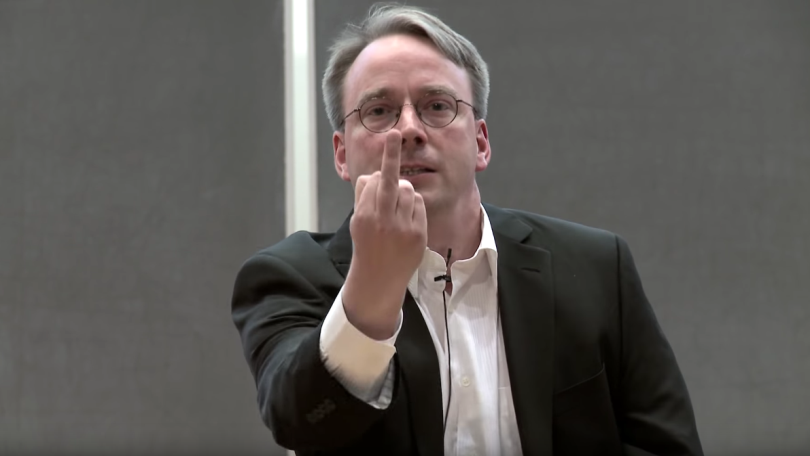
\includegraphics[width=1.0\textwidth]{images/linus.png}
	\end{frame}

	\begin{frame}{Richard Stallman}
		\centering
		
\includegraphics[width=1.0\textwidth]{images/stallman.png}
	\end{frame}

	\section{Co je to Linux?}
	
	\begin{frame}{Linux}
		%https://wiki.swpelc.eu/programming/basics.html

		{\centering \texttt{\href{https://wiki.swpelc.eu/programming/basics.html}{https://wiki.swpelc.eu/programming/basics.html}} \par}		
	\end{frame}

	\section{References}

	\begin{frame}{References}
		{\centering \texttt{\href{https://swpelc.eu}{swpelc.eu}} \par}
		{\centering \texttt{\href{https://wiki.swpelc.eu}{wiki.swpelc.eu}} \par}
	\end{frame}

\end{document}